\documentclass[UTF8,a4paper,12pt]{ctexart}
\usepackage{geometry}
\usepackage{graphicx}
\usepackage{booktabs}
\usepackage{hyperref}
\usepackage{amsmath}
\usepackage{float}
\usepackage{xcolor}
\geometry{left=2.5cm,right=2.5cm,top=2.5cm,bottom=2.5cm}

\hypersetup{
    colorlinks=true,
    linkcolor=blue,
    urlcolor=blue,
    citecolor=blue
}

\title{课程作业一与作业二实验报告}
\author{姓名：\underline{\hspace{4cm}} \quad 学号：\underline{\hspace{4cm}}}
\date{\today}

\begin{document}
\maketitle

\section{作业一：三层神经网络地表覆盖分类}

\subsection{任务目标}

作业一基于 EuroSAT RGB 遥感图像数据集，从零开始实现一个三层全连接神经网络分类器，对地表覆盖类型进行 10 类分类。该作业不使用 PyTorch、TensorFlow 等深度学习框架，而是使用 NumPy 手工实现数据读取、前向传播、Softmax 交叉熵损失、反向传播、mini-batch 梯度下降和模型评估。

\subsection{数据集与预处理}

EuroSAT RGB 数据集共包含 27000 张遥感图像，每张图像大小为 $64\times64$，共 10 个类别：AnnualCrop、Forest、HerbaceousVegetation、Highway、Industrial、Pasture、PermanentCrop、Residential、River 和 SeaLake。实验采用分层划分方式，将数据集划分为训练集、验证集和测试集，比例为 70\%、15\% 和 15\%，对应样本数分别为 18900、4050 和 4050。

由于从零实现的 MLP 直接处理 $64\times64\times3=12288$ 维输入成本较高，实验将图像缩放到 $16\times16$，保留 RGB 三通道并展平为 768 维向量。随后将像素值归一化到 $[0,1]$，并使用训练集均值和标准差对训练集、验证集与测试集进行标准化。

\subsection{模型结构与训练设置}

作业一模型为三层全连接神经网络，结构如下：

\[
768 \rightarrow 256 \rightarrow 128 \rightarrow 10
\]

两个隐藏层使用 ReLU 激活函数，输出层使用 Softmax 得到 10 类概率分布。损失函数为多分类交叉熵，参数初始化采用适合 ReLU 的 He 初始化。训练采用 mini-batch 梯度下降，并在每个 epoch 后使用验证集评估模型，最终保存验证集准确率最高的模型参数。

\begin{table}[H]
\centering
\begin{tabular}{lc}
\toprule
参数 & 取值 \\
\midrule
输入尺寸 & $16\times16\times3=768$ \\
隐藏层维度 & 256, 128 \\
输出类别数 & 10 \\
学习率 & 0.03 \\
Batch size & 512 \\
Epoch & 20 \\
最佳 epoch & 19 \\
\bottomrule
\end{tabular}
\caption{作业一 MLP 训练配置}
\label{tab:hw1_config}
\end{table}

\subsection{实验结果}

作业一最终使用验证集最优模型进行测试，测试集准确率为 61.78\%，Macro F1 为 61.23\%。训练曲线如图\ref{fig:hw1_training_curves} 所示，可以看到训练和验证准确率整体上升，loss 整体下降，但验证集在后期仍存在一定波动，因此保存验证集最佳模型是必要的。

\begin{table}[H]
\centering
\begin{tabular}{lc}
\toprule
指标 & 数值 \\
\midrule
训练集准确率 & 65.92\% \\
验证集准确率 & 61.33\% \\
测试集准确率 & 61.78\% \\
测试集损失 & 1.0807 \\
Macro Precision & 61.45\% \\
Macro Recall & 61.84\% \\
Macro F1 & 61.23\% \\
\bottomrule
\end{tabular}
\caption{作业一测试结果}
\label{tab:hw1_metrics}
\end{table}

\begin{figure}[H]
\centering
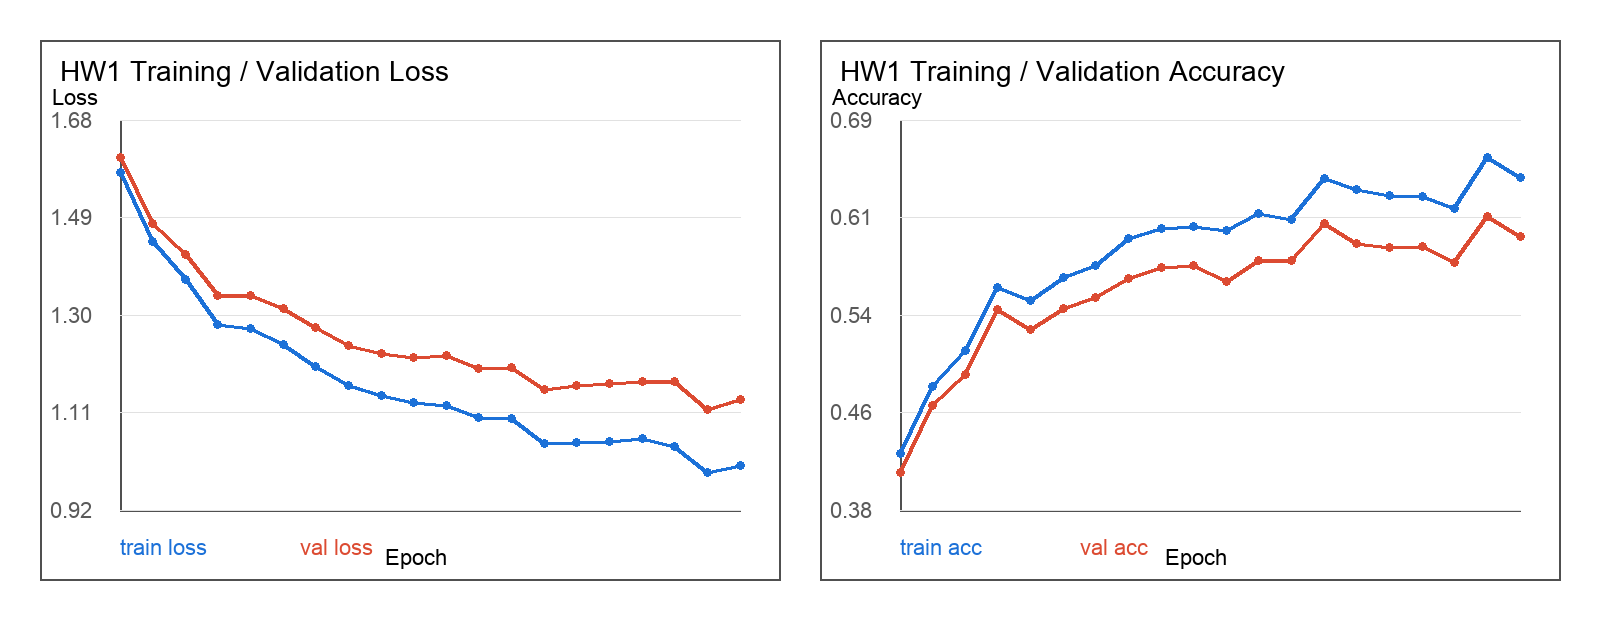
\includegraphics[width=0.95\linewidth]{figures/hw1_training_curves.png}
\caption{作业一训练与验证曲线}
\label{fig:hw1_training_curves}
\end{figure}

从分类结果看，模型在 Industrial、SeaLake 和 Forest 等类别上表现较好，说明这些类别在颜色和整体纹理上区分度更高；在 Highway、PermanentCrop 等类别上表现较弱，主要原因是这些类别与农作物、草地、河流等场景存在较强视觉相似性。此外，MLP 将图像展平为向量后会丢失局部空间结构，不如卷积神经网络擅长提取邻域纹理和形状特征。

\begin{figure}[H]
\centering
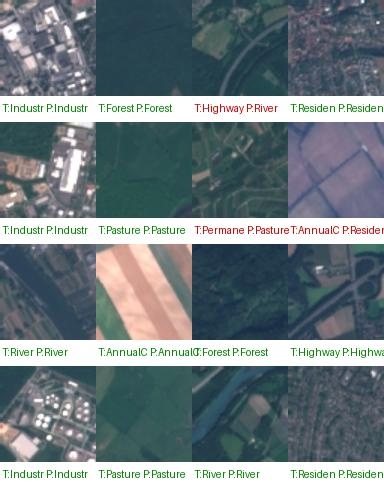
\includegraphics[width=0.9\linewidth]{figures/hw1_prediction_grid.jpg}
\caption{作业一测试样例预测可视化}
\label{fig:hw1_prediction_grid}
\end{figure}

\section{作业二：场景目标检测与视频多目标跟踪}

本实验面向道路交通场景，完成车辆目标检测、视频多目标跟踪、遮挡场景下的 Tracking ID 分析以及车辆越线计数。实验首先使用 Road Vehicle Images Dataset 微调 YOLOv8 单阶段目标检测模型，得到面向道路车辆类别的专属检测模型；随后将训练后的模型应用于自采集道路视频，对视频逐帧进行车辆检测，并结合 ByteTrack 跟踪算法为每个目标分配稳定的 Tracking ID。最后，本文在视频画面中设置虚拟计数线，根据目标中心点轨迹统计跨线车辆数量。

\section{数据集与模型}

\subsection{数据集}

本实验使用 Road Vehicle Images Dataset。该数据集包含道路交通场景中的多类车辆图像及 YOLO 格式边界框标注。实验中将数据集整理为 YOLOv8 所需目录结构，其中训练集与验证集分别位于 \texttt{images/train}、\texttt{images/val}，对应标注位于 \texttt{labels/train}、\texttt{labels/val}。

数据集包含多种道路目标类别，例如 truck、rickshaw、auto rickshaw、bicycle、scooter、minibus、policecar 等。由于类别数量较多，且部分类别样本较少，整体检测指标会受到类别不均衡、小目标和遮挡等因素影响。

\subsection{检测模型}

本实验采用 YOLOv8s 作为基础检测模型。YOLOv8 属于单阶段目标检测器，能够直接从输入图像预测目标类别、置信度和边界框。相比两阶段检测器，YOLO 系列模型具有推理速度快、部署简单的特点，适合用于视频逐帧目标检测。

本次选择 YOLOv8s 的原因如下：

\begin{itemize}
    \item 模型规模适中，参数量约 1113 万，权重文件约 21 MB；
    \item 相比 YOLOv8n，YOLOv8s 具有更好的检测精度；
    \item 相比 YOLOv8m/l/x，YOLOv8s 对本机训练和推理更友好；
    \item 能够在本机 Apple M4 Pro 的 MPS 后端完成微调训练。
\end{itemize}

\section{实验设置}

\begin{table}[H]
\centering
\begin{tabular}{ll}
\toprule
项目 & 设置 \\
\midrule
模型 & YOLOv8s \\
预训练权重 & \texttt{yolov8s.pt} \\
训练设备 & Apple M4 Pro, MPS 后端 \\
输入尺寸 & 512 \\
Batch size & 4 \\
Epoch & 30 \\
优化器 & Ultralytics auto optimizer（AdamW） \\
损失函数 & Box loss + Classification loss + DFL loss \\
评价指标 & Precision, Recall, mAP50, mAP50-95 \\
实验可视化 & SwanLab \\
\bottomrule
\end{tabular}
\caption{模型训练配置}
\label{tab:train_config}
\end{table}

训练过程使用 SwanLab 记录实验曲线，包括训练集损失、验证集损失、Precision、Recall、mAP50 与 mAP50-95 等指标。SwanLab 实验地址为：
\url{https://swanlab.cn/@cywsds090/hw2-road-vehicle-yolov8/runs/ln5axo7d2ai1ab88955wn}。

\section{训练结果}

本次训练共进行 30 个 epoch，总训练耗时约 3.67 小时。最终模型保存为 \texttt{best.pt}，权重文件大小约 21 MB。最终验证结果如表\ref{tab:metrics} 所示。

\begin{table}[H]
\centering
\begin{tabular}{lc}
\toprule
指标 & 数值 \\
\midrule
Precision & 0.609 \\
Recall & 0.424 \\
mAP50 & 0.457 \\
mAP50-95 & 0.282 \\
\bottomrule
\end{tabular}
\caption{验证集整体检测结果}
\label{tab:metrics}
\end{table}

训练过程可视化曲线如图\ref{fig:training_curves} 所示。可以看到，训练后期 box loss、classification loss 与 DFL loss 整体下降，mAP 指标逐步提升，说明模型在道路车辆检测任务上完成了有效微调。

\begin{figure}[H]
\centering
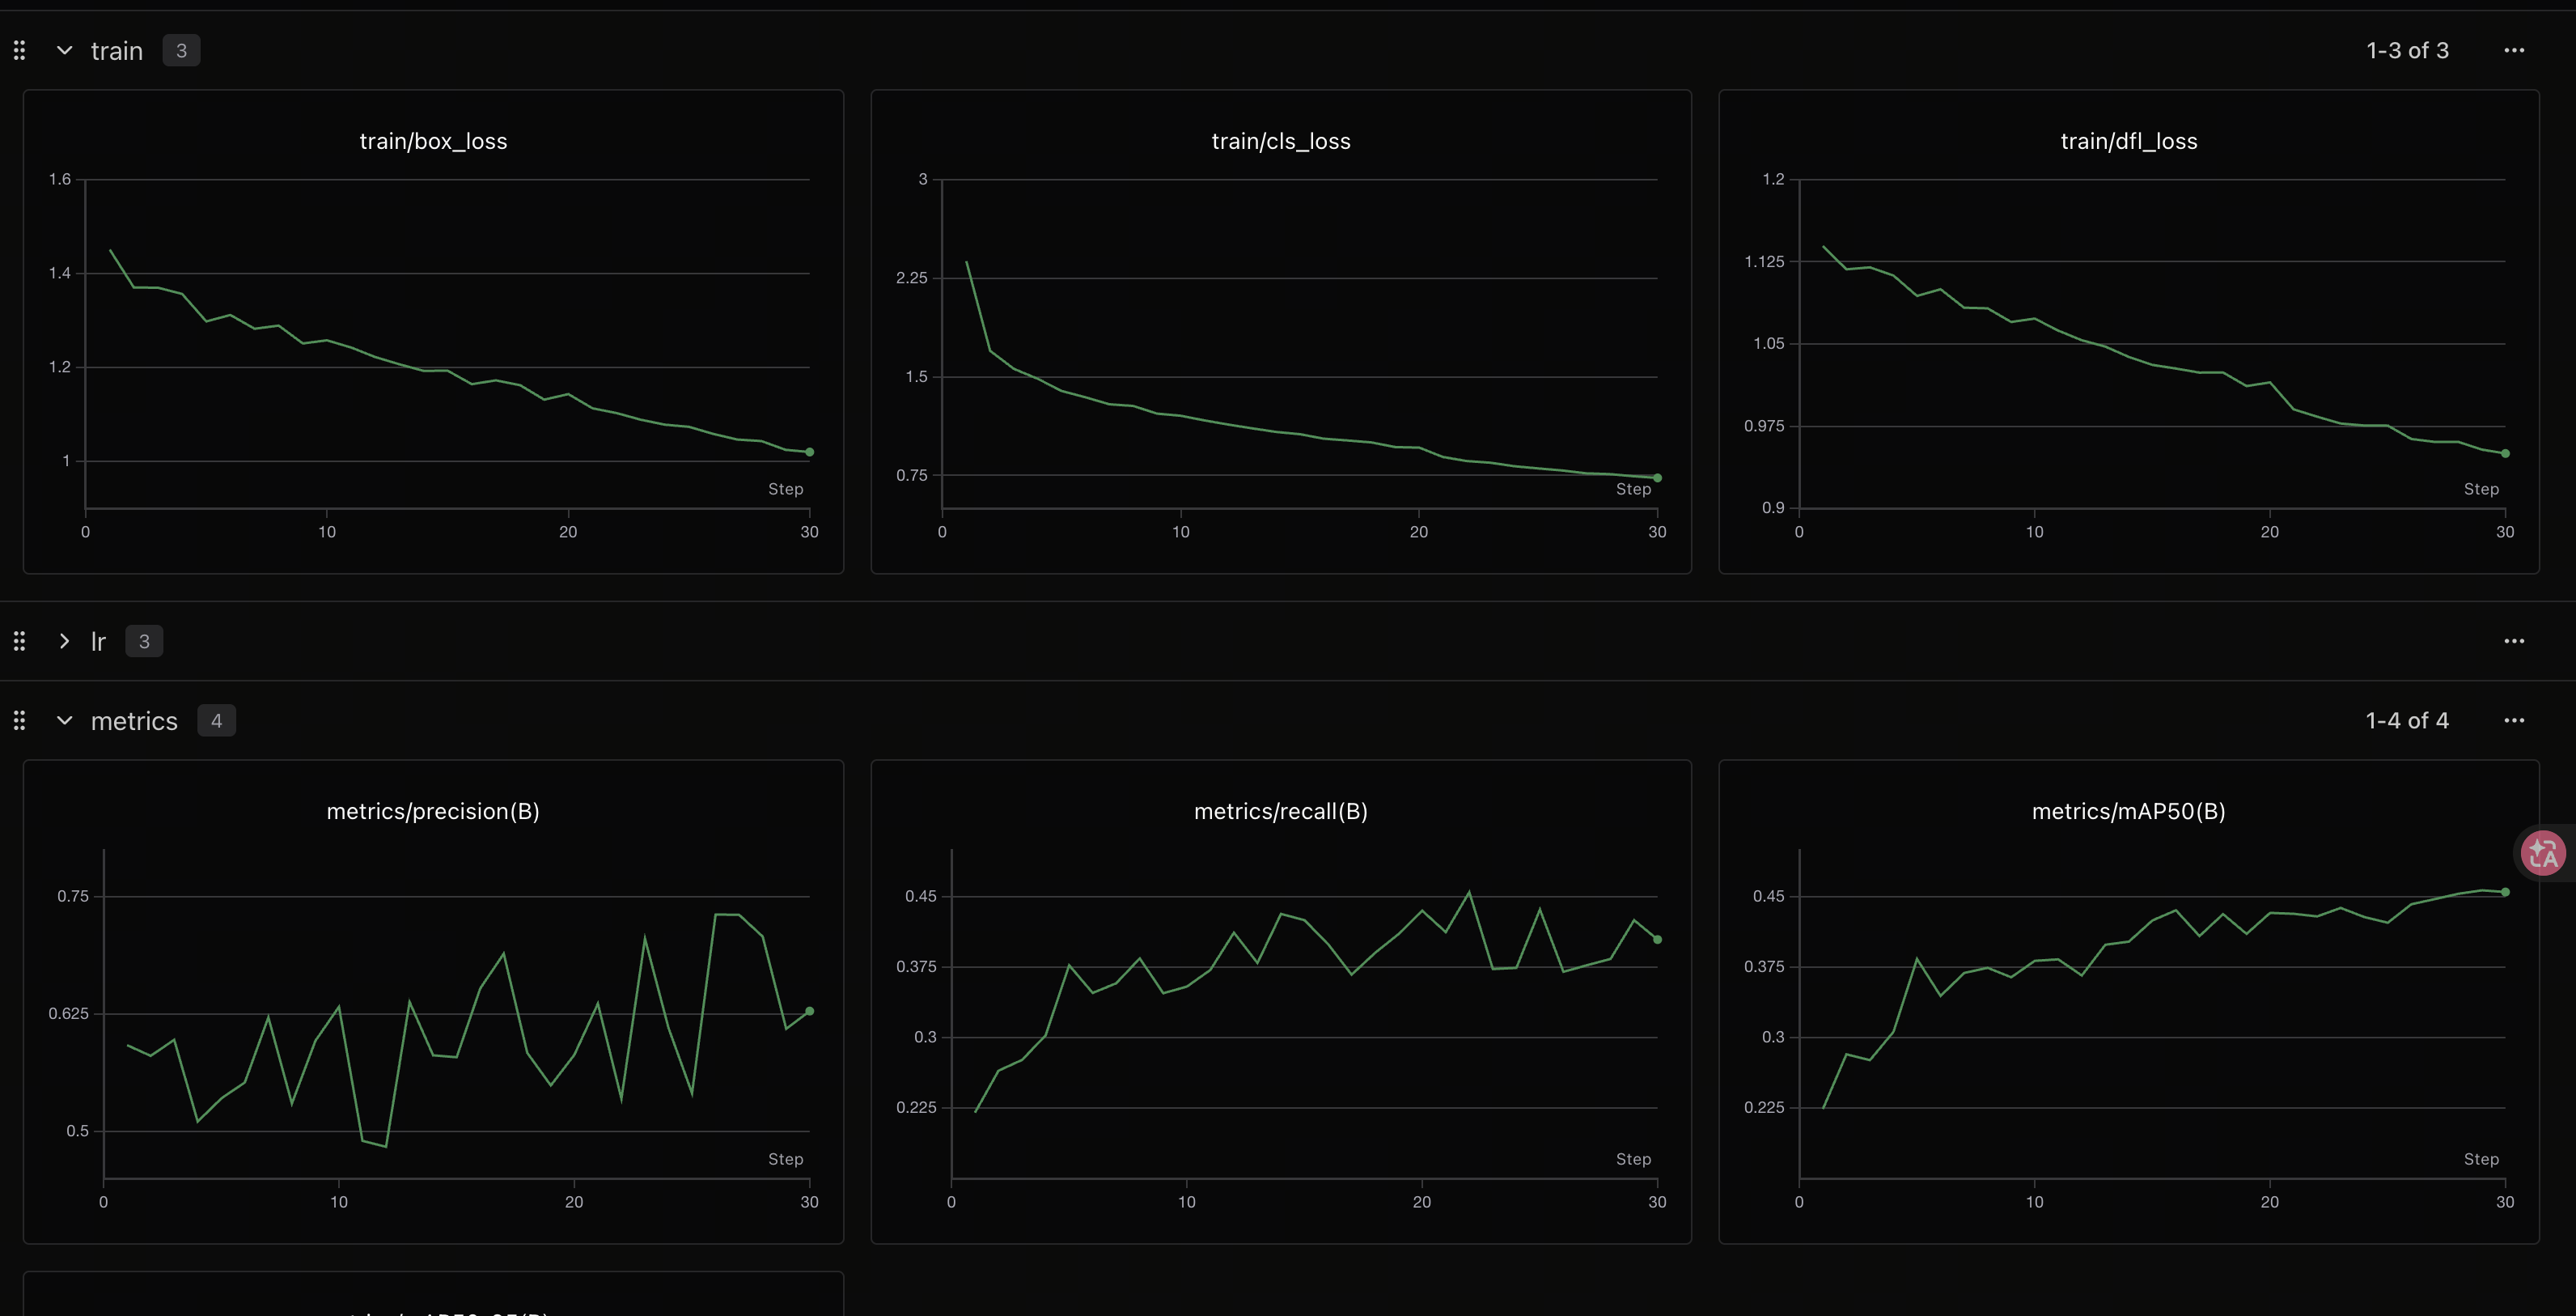
\includegraphics[width=0.95\linewidth]{figures/swanlab_curves.png}
\caption{SwanLab 训练过程可视化曲线}
\label{fig:training_curves}
\end{figure}

\section{视频检测与多目标跟踪}

测试视频为自采集道路场景视频，视频分辨率为 1280$\times$720，帧率为 30 FPS，共 788 帧，时长约 26.3 秒。拍摄时相机保持固定，画面中存在道路车辆、中央路牌和杆件等固定遮挡物，适合用于测试检测、跟踪和遮挡场景下的 ID 稳定性。

视频检测与跟踪流程如下：

\begin{enumerate}
    \item 使用训练后的 \texttt{best.pt} 对视频逐帧进行车辆检测；
    \item 使用 YOLOv8 的 tracking 接口结合 ByteTrack 跟踪器，为连续帧中的目标分配 Tracking ID；
    \item 在视频中绘制检测框、类别、Tracking ID、运动轨迹和虚拟计数线；
    \item 输出带可视化结果的视频和轨迹 CSV 文件。
\end{enumerate}

由于中央路牌属于固定物体，模型在个别帧中会将其误检为车辆。为避免固定误检影响展示和计数，实验中对中央路牌区域设置了忽略区域，仅保留道路区域中的车辆目标。检测与跟踪结果示例如图\ref{fig:tracking_frame} 所示。

\begin{figure}[H]
\centering
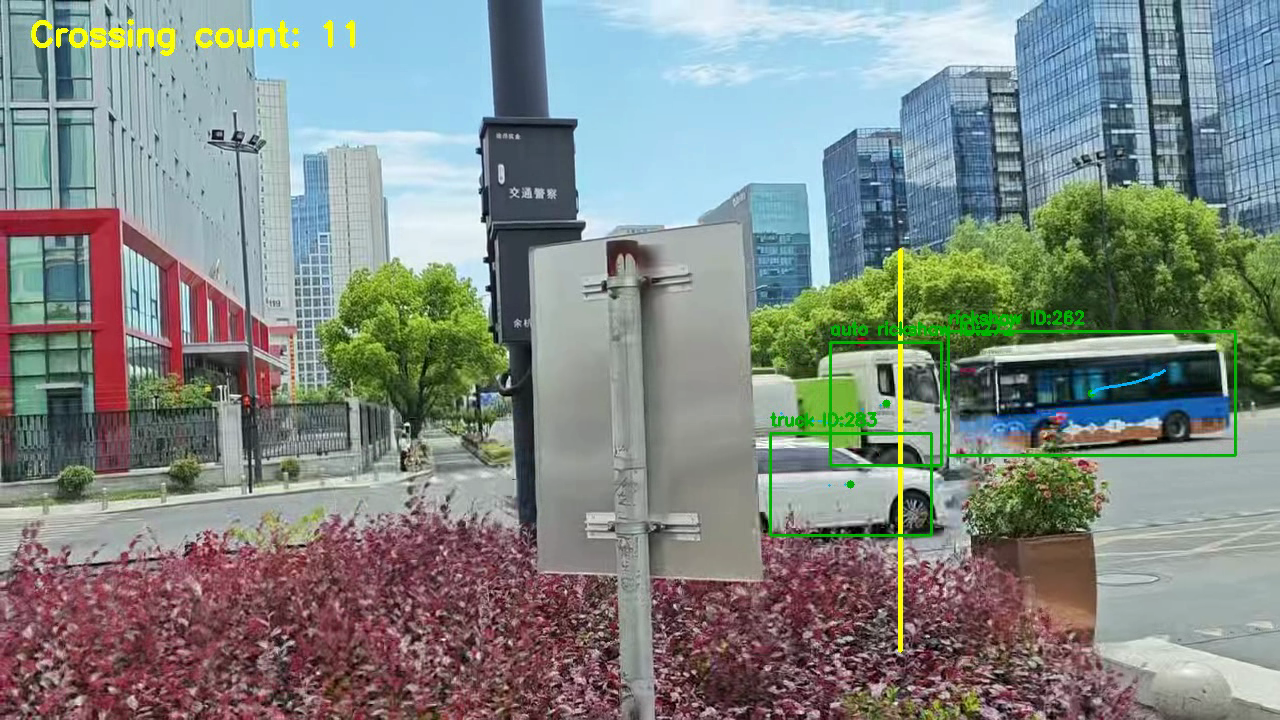
\includegraphics[width=0.95\linewidth]{figures/tracking_frame.png}
\caption{视频车辆检测与多目标跟踪结果示例}
\label{fig:tracking_frame}
\end{figure}

\section{遮挡与 ID 跳变分析}

遮挡是多目标跟踪中的典型难点。本实验视频中，车辆经过中央路牌、杆件和绿化遮挡区域时，检测框可能被部分遮挡，甚至在短时间内消失。图\ref{fig:occlusion_frames} 展示了车辆经过遮挡区域附近的连续片段。

\begin{figure}[H]
\centering
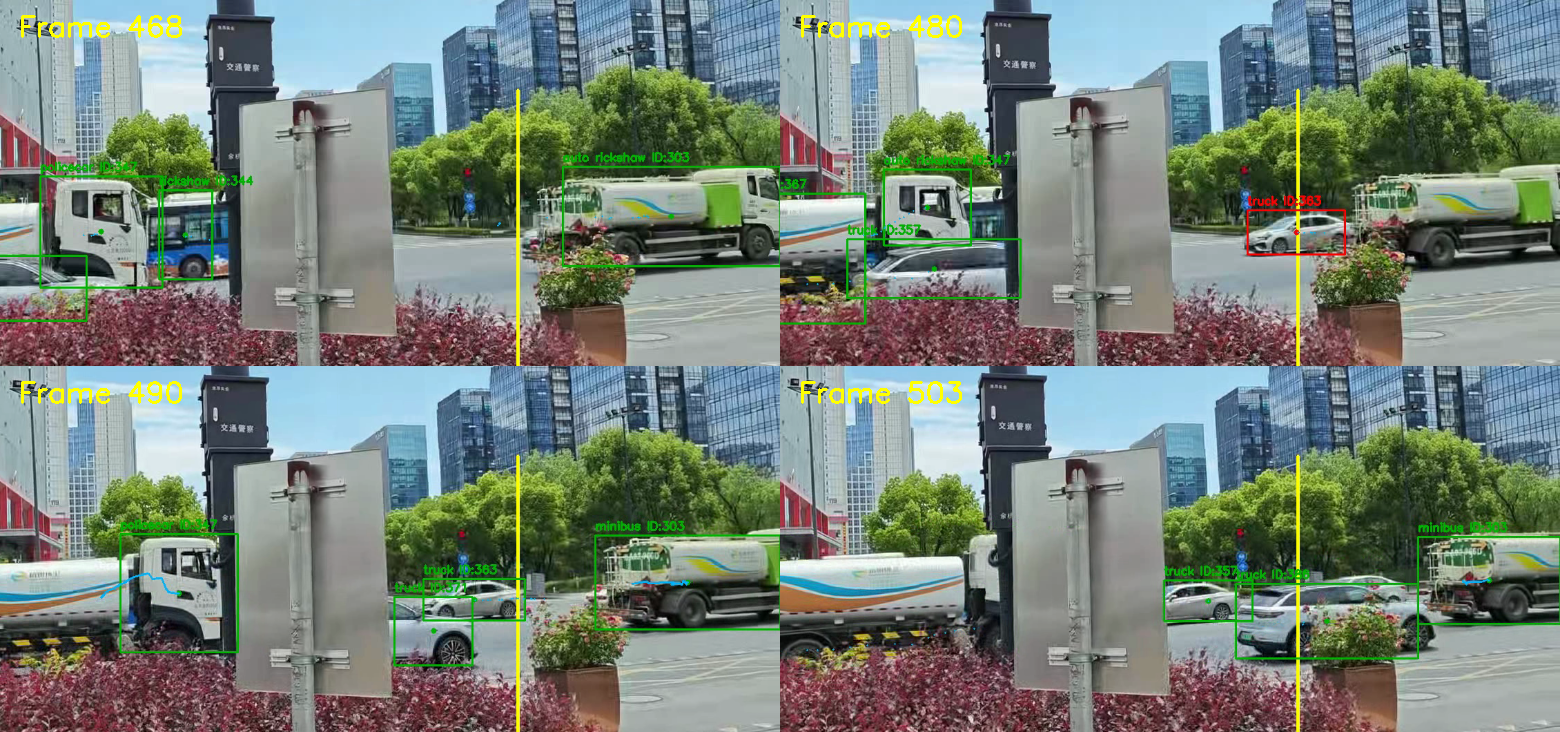
\includegraphics[width=0.98\linewidth]{figures/occlusion_frames.png}
\caption{遮挡区域附近的连续帧跟踪结果}
\label{fig:occlusion_frames}
\end{figure}

从图中可以观察到，部分车辆在遮挡和密集交汇场景下仍能保持连续轨迹，但也存在 ID 不稳定的风险。例如，当车辆被中央路牌或前景绿化部分遮挡时，检测器可能无法连续输出完整目标框；若目标重新出现时与其他车辆距离较近，跟踪器可能将其分配为新的 ID，形成 ID switch。该现象说明多目标跟踪不仅依赖检测精度，还依赖相邻帧之间的位置连续性和目标匹配质量。

因此，本实验中遮挡分析的结论为：短时间、轻度遮挡时，跟踪器通常可以维持较稳定的 Tracking ID；当目标被较大面积遮挡、与其他车辆重叠或检测框置信度下降时，可能出现目标丢失或 ID 跳变。

\section{越线计数}

为统计视频中经过指定区域的车辆数量，实验在画面右侧道路区域设置一条竖直虚拟线，端点坐标为 $(900,250)$ 与 $(900,650)$。对每个 Tracking ID，记录其检测框中心点轨迹。当同一个 Tracking ID 的中心点从虚拟线一侧移动到另一侧时，判定该车辆完成一次越线。为避免重复统计，同一个 Tracking ID 只计数一次。

设虚拟线两端点为 $(x_1,y_1)$ 与 $(x_2,y_2)$，目标中心点为 $(c_x,c_y)$，使用叉积符号判断中心点位于直线哪一侧：

\[
s=(x_2-x_1)(c_y-y_1)-(y_2-y_1)(c_x-x_1)
\]

若同一目标在相邻帧中的 $s$ 符号发生变化，则判定其跨越虚拟线。最终本测试视频统计得到越线车辆数为 22，结果示例如图\ref{fig:line_counting} 所示。

\begin{figure}[H]
\centering
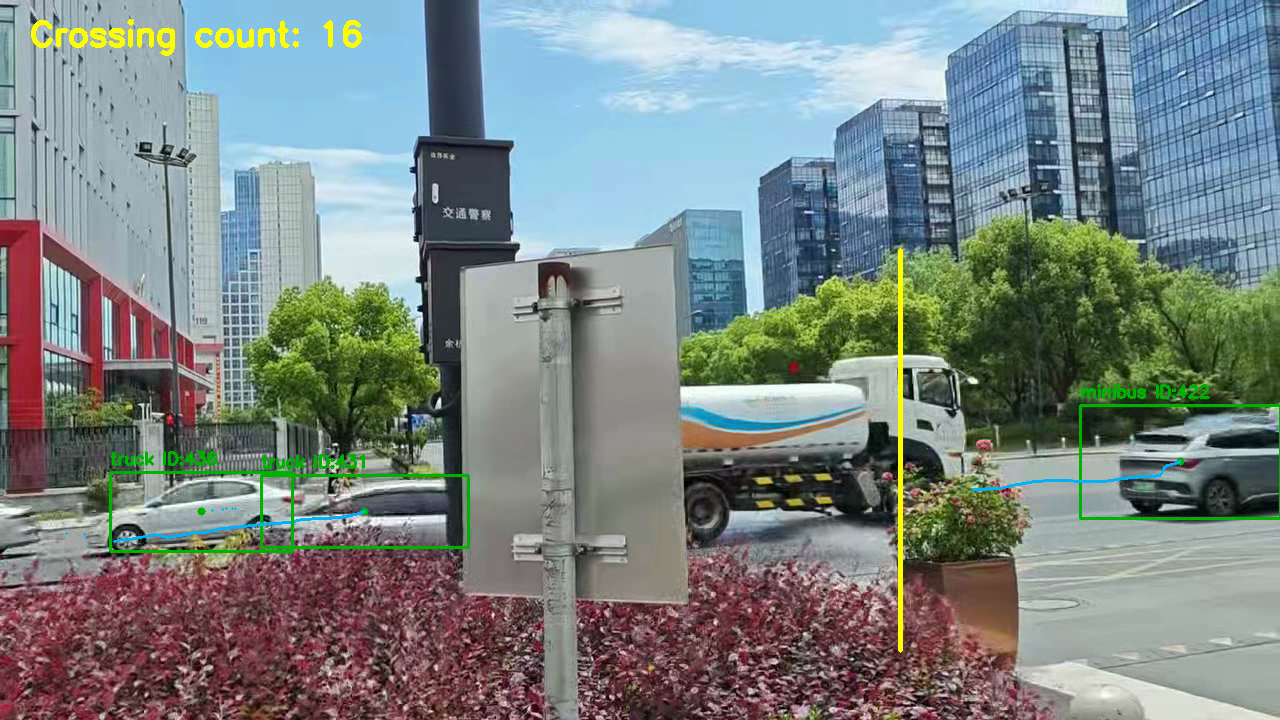
\includegraphics[width=0.95\linewidth]{figures/line_counting.png}
\caption{虚拟线越线计数结果示例}
\label{fig:line_counting}
\end{figure}

\section{实验文件与复现说明}

作业一主要代码与结果文件如下：

\begin{itemize}
    \item \texttt{/Users/bytedance/Private\_Czw/homework/hw1/train\_mlp.py}：NumPy 三层 MLP 训练、验证与测试脚本；
    \item \texttt{/Users/bytedance/Private\_Czw/homework/hw1/outputs\_final/metrics.json}：作业一最终训练配置与测试指标；
    \item \texttt{/Users/bytedance/Private\_Czw/homework/hw1/outputs\_final/model\_weights.npz}：作业一验证集最优模型参数。
\end{itemize}

作业二主要代码文件如下：

\begin{itemize}
    \item \texttt{scripts/prepare\_road\_vehicle\_dataset.py}：下载并整理数据集；
    \item \texttt{scripts/train\_local.py}：在本机 MPS/CPU 环境训练 YOLOv8；
    \item \texttt{scripts/train\_a100.py}：在 A100 GPU 环境训练 YOLOv8；
    \item \texttt{scripts/track\_count\_line.py}：执行视频跟踪、ID 可视化和越线计数；
    \item \texttt{report/main.tex}：实验报告源码。
\end{itemize}

训练后的模型权重位于：

\begin{center}
\texttt{runs/detect/runs\_local/road\_vehicle\_yolov8s\_local\_cpu/weights/best.pt}
\end{center}

视频输出结果位于：

\begin{center}
\texttt{outputs/tracked\_counted\_clean.mp4}
\end{center}

\textbf{代码与模型权重链接：}根据课程要求，实验代码已上传至 public GitHub repo，训练好的 HW2 YOLOv8s 权重已上传至百度网盘。

\begin{itemize}
    \item GitHub repo：\url{https://github.com/cywpsms090/fudan_CS60003_hw.git}
    \item 模型权重网盘链接：\url{https://pan.baidu.com/s/1SNRlUiKycskM1eQ0Y6ZJhg}，提取码：\texttt{ggbe}
\end{itemize}

\section{结论}

作业一完成了基于 NumPy 的三层全连接神经网络实现，并在 EuroSAT RGB 遥感图像数据集上完成地表覆盖 10 分类。实验结果表明，即使不使用深度学习框架，手写 MLP 也能够完成完整的前向传播、反向传播和多分类训练流程，最终测试集准确率达到 61.78\%。但由于 MLP 将图像展平为一维向量，对局部空间结构利用不足，因此在 Highway、PermanentCrop 等视觉相似类别上表现有限。

作业二完成了基于 YOLOv8s 的道路车辆检测模型微调，并将训练后的模型应用于自采集道路视频，实现了车辆检测、多目标跟踪、遮挡场景分析和越线计数。实验结果表明，YOLOv8s 在本任务中能够检测常见道路车辆，并结合 ByteTrack 为视频中的车辆分配 Tracking ID。测试视频中最终统计得到 22 次车辆越线。

两次作业体现了从基础神经网络到现代计算机视觉模型的递进关系：作业一侧重理解神经网络训练的基本机制，作业二侧重使用现代单阶段检测模型解决实际视频场景问题。作业二仍存在一定局限性：首先，车辆数据集中类别较多且不均衡，部分类别样本较少，影响整体 mAP；其次，固定遮挡物和复杂道路背景可能引入误检；最后，在车辆密集交汇或被遮挡时间较长时，Tracking ID 可能发生跳变。后续可以通过增加训练数据、提高输入分辨率、使用更大模型或调整跟踪器参数进一步提升检测与跟踪稳定性。

\end{document}
